% \documentclass[10pt]{beamer}
\documentclass[aspectratio=169, 10pt]{beamer}

\usetheme{metropolis}
\usepackage{appendixnumberbeamer}

\usepackage{booktabs}
\usepackage[scale=2]{ccicons}
\usepackage{natbib}

\usepackage{pgfplots}
\usepgfplotslibrary{dateplot}

\usepackage{xspace}
\newcommand{\themename}{\textbf{\textsc{metropolis}}\xspace}

\usepackage{amsmath, amsthm, amssymb, mathtext}
\usepackage{unicode-math}
\usepackage[english, russian]{babel}
\usepackage{tabularx} % таблицы
\usepackage{fancybox, fancyhdr}
\usepackage{ulem, color, tcolorbox, graphicx}
% \usepackage[dvips, xelatex]{graphicx}
% \usepackage{graphicx}
% \usepackage{ifpdf,mla}
\usepackage{float, wrapfig, subcaption}
\usepackage{enumerate} % дополнительный функционал для списков
\usepackage{multicol} % разделение на несколько колонок
\usepackage{ifthen} % условия
\usepackage{physics} % содержит дифференциальные операторы (\dd, \dv, \pdv и т. д.) и не только

\definecolor{hSum1}{HTML}{188F1A}
\definecolor{hSum2}{HTML}{185F1A}
\definecolor{hDif1}{HTML}{CC1818}
\definecolor{hDif2}{HTML}{9C1818}

% вертикальное выравнивание колонок в таблице
\renewcommand\tabularxcolumn[1]{m{#1}}

\DeclareMathAlphabet{\mathcal}{OMS}{cmsy}{m}{n}
\let\mathbb\relax % remove the definition by unicode-math
\DeclareMathAlphabet{\mathbb}{U}{msb}{m}{n}

\defaultfontfeatures{Ligatures=TeX}
\newcommand{\import}[1]{\input{../../commands/#1}} % импорт из папки commands

% \newfontfamily\accuratist{Accuratist}

% настройка изображений
% \DeclareGraphicsExtensions{.pdf,.png,.jpg}
\graphicspath{{./img/}}

\Russian

\import{textCommands}            % текстовые команды
\import{mathCommands}            % математические команды
\import{RUSmathCommands}         % особенности русской типографии
\import{linearAlgebraCommands}   % линейная алгебра
\import{setsAndDiscreteCommands} % множества и дискретная математика

\newcommand{\signal}{S}
\newcommand{\DWT}{\operatorname{W}}
\newcommand{\thresh}[1]{\operatorname{F}_{#1}}

\begin{document}
	\nocite{*}
	% \setbeamertemplate{footline}{\insertframenumber/\inserttotalframenumber}
	\begin{frame}[plain]{Актуальные проблемы современного строительства}
	  \setbeamertemplate{section in toc}[sections numbered]
	  % \tableofcontents[hideallsubsections]
	  \begin{center}%
	    Санкт-Петербургский политехнический университет Петра великого \\ 
	    Институт компьютерных наук и технологий \\ 
	    Кафедра компьютерных интеллектуальных технологий
	  \end{center}
	  \vfill
	  \begin{center}%
	    \huge\bf
	    Сжатие изображений с помощью \\ вейвлет-преобразования
	  \end{center}
	  \vfill
	  \begin{tabularx}{\textwidth}{CC}%
	    Выполнили:                               & Научный руководитель: \\ 
	    \textbf{Ксенофонтова Вера} (гр. 23536/1) & доцент кафедры <<Высшая математика>> \\
	    \textbf{Фурман Владислав} (гр. 23536/2)  & \textbf{Филимоненкова Надежда Викторовна}
	  \end{tabularx}%

	\end{frame}

	\begin{frame}{Цели и задачи проекта}%
	  \ul{
	    % \item обзор теории вейвлет-преобразований сингалов;
	    % \item моделирование этапа сжатия изображения, а также алгоритма устранения шума с помощью вейвлета \code{D4};
	    % \item анализ полученных результатов сжатия конкретных изображений, сравнение со сжатием с помощью косинус-преобразования Фурье (\code{DCT}).
	    \item Изучение вейвлет-преобразования;
	    \item моделирование этапа сжатия изображения с помощью вейвлетов Добеши;
	    \item анализ полученных результатов сжатия конкретных изображения, сравнение со сжатием с помощью косинус-преобразования Фурье (\code{DCT}).
	  }
	\end{frame}

	\begin{frame}{Задача аппроксимации в непрерывном случае}%
		
		Нередко возникает необходимость аппроксимировать сложновычислимую функцию более простой.
		Для этого её можно разложить в ряд Фурье по ортонормированному базису $ \qty{e_k(x)}_{k=1}^{\infty} $:
		\begin{equation}
			f(x) = \ser c_k e_k(x), \quad c_k = (f, e_k)
		\end{equation}
		После чего взять конечное число членов ряда:
		\begin{equation}
			f(x) \approx \sm{n} c_k e_k(x), \quad c_k = (f, e_k)
		\end{equation}
		Обычно рассматривают пространство $ L^2 (0; 1) $, где скалярное произведение есть интеграл:
		\begin{equation}
			(f, e_k) = \dint{0}{1}{f(x) e_k(x)}
		\end{equation}

		% англ. wavelet --- маленькая, короткая волна;

		% \begin{equation}%
		% 	\psi_{ab} (t) = \oo{\sqrt{|a|}} \psi \qty(\ov{t - b}{a}), \quad (a, b) \in \R, \quad \psi (t) \in L^2 (\R),
		% \end{equation}
		% \ul{
		% 	\item $ \psi (t) $ --- материнский вейвлет;
		% 	\item $ b $ --- сдвиг по времени $ b $;
		% 	\item $ a $ --- изменения временного масштаба;
		% 	\item $ 1/\sqrt{|a|} $ --- множитель, обеспечивающий независимость нормы функций от масштабирующего числа.
		% }
	\end{frame}

	\begin{frame}{Система косинусов}%
		Одним из наиболее распространнёных базисов в $L^2 (0; 1)$ является система косинусов:
		\begin{equation}
			\sq{\cos(k \pi x)}
			= \qty{\cos(\pi x), \ \cos(2 \pi x), \ \cos(3 \pi x), \ \ldots}
		\end{equation}
		\begin{center}%
			\includegraphics[width=6cm]{cos.pdf}
		\end{center}
	\end{frame}

	\begin{frame}{Системы вейвлетов}%
		Но есть и другие базисы — вейвлеты, графики которых представляют собой <<всплески>> на коротком промежутке.
		\begin{center}%
			\includegraphics[scale=0.5]{wavelets.png}
		\end{center}
	\end{frame}

	% \begin{frame}{Свойства вейвлетов}%
	% 	\textbf{Так, ну это, я думаю, можно убрать, это всё-равно никто не запомнит.}

	% 	\ul{
	% 		\item локализация,
	% 		\item нулевое среднее значение:
	% 			\begin{equation}%
	% 				\dint[t]{-\infty}{\infty}{\psi (t)} = 0,
	% 			\end{equation}
	% 		\item ограниченность:
	% 			\begin{equation}%
	% 				\norm{\psi(t)}^2 = \dint[t]{-\infty}{\infty}{|\psi(t)|^2} < \infty,
	% 			\end{equation}
	% 		\item самоподобие.
	% 	}
	% \end{frame}

	% {
		% \usebackgroundtemplate{\includegraphics[width=\paperwidth]{cmp2.png}}
		% \begin{frame}{Применение вейвлетов при сжатии данных}%
		% 	\begin{center}%
		% 		\includegraphics[scale=0.2]{cmp2.png}
		% 		% \includegraphics[scale=0.33]{comp.jpg}
		% 	\end{center}
		% \end{frame}
	% }

	% \begin{frame}{Вейвлет-преобразование}%
	% 	\textbf{Не, это тоже что-то не то, уберём, наверное.}

	% 	\textbf{Вейвлет-преобразование} (\code{WT}) --- интегральное преобразование, которое представляет собой свертку вейвлет-функции с сигналом, переводящее сигнал из временного представления в частотно-временное: 
	% 	\textbf{Вейвлет-преобразование} --- удобный и эффективный инструмент для обработки сигналов и функций, нестационарных во времени или неоднородных в пространстве, то есть требующих анализа сразу в двух измерениях.

	% 	\textbf{Результат}: апрокисимирующая и детализирующая составляющие.
	% 	\culs{
	% 		\item дискретное (\code{DWT}),
	% 		\item непрерывное (\code{CWT}).
	% 	}
	% 	\begin{center}%
	% 		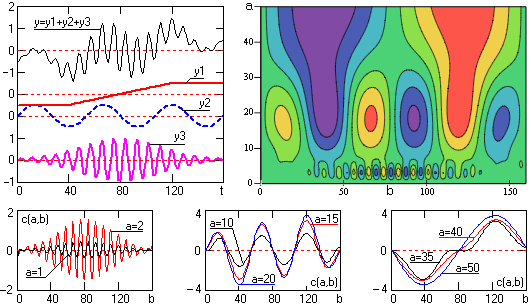
\includegraphics[scale=0.45]{transform.png}
	% 	\end{center}
	% \end{frame}

	\begin{frame}{Переход к дискретному случаю}%
		% Переход от преобразования непрерывного к преобразованию дискретному происходит путём замены функции на значения её в конкретных точках. В такой ситуации раскладываемая функция и базисы превращаются в векторы, интеграл превращается в интегральную сумму (я потом допишу, что берётся интеграл для нахождения коэффициентов).
		Заменяем функцию на её значения в конкретных точках (вектор), интеграл --- на интегральную сумму.
		\[
			f(x) \longrightarrow \bx{f_1 & f_2 & f_3 & \ldots & f_n}
		\]
		\[
			e_k(x) \longrightarrow \bx{e_{k, 1} & e_{k, 2} & e_{k, 3} & \ldots & e_{k, n}}
		\]
		\[
			\int \longrightarrow \sum
		\]
		\begin{center}%
			\includegraphics[scale=0.4]{disc.pdf}
		\end{center}
	\end{frame}

	\begin{frame}{О сжатии изображений}%
		Допустим, у нас есть последовательность нулей:
		\begin{equation}
			\und{00 \ 00 \ 00 \ 00 \ 00 \ 00 \ 00 \ 00 \ \ldots \ 00 \ 00 \ 00 \ 00 \ 00 \ 00 \ 00 \ 00}{256},
		\end{equation}
		чтобы записать их как отдельные числа нужно немало памяти, куда эффективнее можно сделать вот так:
		\begin{equation}
			256 \cdot 0,
		\end{equation}
		то есть вместо последовательности нулей будем записывать их \textbf{количество}. Ставим себе цель: получить как можно больше нулей после нашего вейвлет-преобразования (за счёт этого и получается сжатие).
	\end{frame}

	\begin{frame}{Дискретное вейвлет-преобразование. Система функций Хаара}%
		% 1909 г. --- \textbf{Альфред Хаар}
		% \culs{
		% 	\item ортогональны,
		% 	\item обладают компактным носителем,
		% 	\item симметричны,
		% 	\item не являются гладкими.
		% }

		\noindent\begin{tabularx}{\textwidth}{CC}%
			$ {\color{hDif1} \psi}(x) = \cscl{
				1, \ 0 \leq x < 1/2 \\ 
				-1, \ 1/2 \leq x < 1 \\ 
				0, \ x \not\in [0; 1)
			} $
			&
			$ {\color{hSum1} \phi}(x) = \cscl{
				1, \ 0 \leq x < 1 \\
				0, \ x \not\in [0; 1)
			} $
			\\ 
			\includegraphics[width=0.2\textwidth]{psi.pdf}
			\includegraphics[width=0.2\textwidth]{4psi.pdf}
			% \img[0.25]{psi.pdf} \img[0.25]{4psi.pdf}
			&
			\includegraphics[width=0.2\textwidth]{phi.pdf}
			\includegraphics[width=0.2\textwidth]{4phi.pdf}
			% \img[0.25]{phi.pdf}
			% a & b
		\end{tabularx}
		$ S $ --- входной сигнал, вектор (яркости пикселей). Коэффициенты разложения:
		\begin{equation}
			{\color{hSum1} a_i} = \ov{S_{2i} + S_{2i + 1}}{2},
			\quad {\color{hDif1} b_i} = \ov{S_{2i} - S_{2i + 1}}{2}
		\end{equation}

		% \noindent\begin{tabularx}{\textwidth}{CC}%
		% 	\begin{equation}\label{psi}%
		% 		\psi (t) = \begin{cases}%
		% 			1,  & t \in [0; 1/2) \\
		% 			-1, & t \in [1/2; 1) \\
		% 			0,  & t \not\in [0; 1) \\
		% 		\end{cases}
		% 	\end{equation}
		% 	& 
		% 	\includegraphics[scale=0.1]{5-1-2.png}
		% \end{tabularx}
		
	\end{frame}

	\begin{frame}{Пример преобразования Хаара}%
		Рассмотрим вектор:
		\begin{equation}
			S = \qty{10, 10, 11, 12}
		\end{equation}
		разбиваем его на полусуммы $ {\color{hSum1} A} $ и полуразности $ {\color{hDif1} B} $:
		\begin{equation}
			{\color{hSum1} A} = \qty{10, \ 11.5}, \ {\color{hDif1} B} = \qty{0, \ 0.5}
		\end{equation}
		полуразности $ {\color{hDif1} B} $ довольно близки к нулю $ \Ra $ если приравнять их к нулю, ошибка будет незначительной (незаметной для глаза). Полусуммы $ {\color{hSum1} A} $ можно точно так же преобразовать, получив при этом 2 вектора:
		\begin{equation}
			{\color{hSum1} A_1} = \qty{10.75}, \ {\color{hDif1} B_1} = \qty{0.75}
		\end{equation}
		и вновь, если мы обнулим ${\color{hDif1} B_1}$, ошибка будет незначительной, а картинку мы сожмём.
		% \textbf{Брать или не брать?}

		% \begin{center}%
		% 	\includegraphics[scale=0.4]{5-1-3.png}
		% \end{center}
	\end{frame}

	% \begin{frame}{Преобразование Хаара}%
	% 	% \textbf{Так, вот тут про полу-разности и полу-суммы рассказывать будем, в контексте той цели, что нужно получить как можно больше нулей.}
		
	% 	% Разные строчки спасут ваши глазочки — (с) Вера, 2017
	% 	\begin{equation}\label{half}%
	% 		\undt{a_i = \ov{s_{2i} + s_{2i + 1}}{2}}{полусумма}, \quad
	% 		\undt{b_i = \ov{s_{2i} - s_{2i + 1}}{2}}{полуразность},
	% 	\end{equation}
	% 	$ S = \qty{s_i}_{i=1}^{n} $ --- входной сигнал, $ s_i $ --- $ i $-й элемент входного сигнала.

	% 	\ul{
	% 		\item $ \mathcal{A} = \qty{a_i}_{i=1}^{n/2} $ --- огрубленная версия входного сигнала
	% 		\item $ \mathcal{B} = \qty{b_i}_{i=1}^{n/2} $ --- детализирующая информация
	% 	}
	% \end{frame}

	\begin{frame}{Преобразование Хаара в матричной форме}%
		% \textbf{Так, ну тут я тоже немного поменяю кое-что}

		Преобразование Хаара можно записать в матричной форме:
		\begin{equation}\label{haar}%
			\und{\bx{
				{\color{hSum1} 1/2}    & {\color{hSum1} 1/2}    & 0      & 0      & \ldots \\ 
				{\color{hDif1} -1/2}   & {\color{hDif1} 1/2}    & 0      & 0      & \ldots \\
				0      & 0      & {\color{hSum1} 1/2}    & {\color{hSum1} 1/2}    & \ldots \\ 
				0      & 0      & {\color{hDif1} -1/2}   & {\color{hDif1} 1/2}    & \ldots \\ 
				\vdots & \vdots & \vdots & \vdots & \ddots
			}}{W}
			\und{\bx{s_1 \\ s_2 \\ s_3 \\ s_4 \\ \vdots}}{S}
			= \und{\bx{{\color{hSum1} a_1} \\ {\color{hDif1} b_1} \\ {\color{hSum1} a_2} \\ {\color{hDif1} b_2} \\ \vdots}}{T}, \quad
			W^{-1} \und{\bx{{\color{hSum1} a_1} \\ {\color{hDif1} b_1} \\ {\color{hSum1} a_2} \\ {\color{hDif1} b_2} \\ \vdots}}{T}
			= \und{\bx{s_1 \\ s_2 \\ s_3 \\ s_4 \\ \vdots}}{S},
		\end{equation}
		здесь $ T $ --- преобразованный сигнал,

		группируем коэффициенты $ {\color{hSum1} a} $ и $ {\color{hDif1} b} $, применяем преобразование к полусуммам $ {\color{hSum1} a} $, пока это возможно,

		заметим, что если поделить матрицу $ W $ на $ \sqrt{2} $, то получится \textbf{ортогональная} матрица,
		\begin{equation}\label{inv}%
			\Ra \qty(\oo{\sqrt{2}}W)^{-1} = \qty(\oo{\sqrt{2}}W)\T
		\end{equation}
	\end{frame}

	\begin{frame}{Двумерное преобразование}%
		% \textbf{Мде, выглядит страшновато, надо будет сделать покрасивше}

		\[
			\bx{
				s_{11} & s_{12} & s_{13} & s_{14} & \ldots \\ 
				s_{21} & s_{22} & s_{23} & s_{24} & \ldots \\ 
				s_{31} & s_{32} & s_{33} & s_{34} & \ldots \\ 
				s_{41} & s_{42} & s_{43} & s_{44} & \ldots \\ 
				\vdots & \vdots & \vdots & \vdots & \ddots
			} \to \undln{\bx{
				{\color{hSum1} a_{11}} & {\color{hDif1} b_{11}} & {\color{hSum1} a_{12}} & {\color{hDif1} b_{12}} & \ldots \\ 
				{\color{hSum1} a_{21}} & {\color{hDif1} b_{21}} & {\color{hSum1} a_{22}} & {\color{hDif1} b_{22}} & \ldots \\ 
				{\color{hSum1} a_{31}} & {\color{hDif1} b_{31}} & {\color{hSum1} a_{32}} & {\color{hDif1} b_{32}} & \ldots \\ 
				{\color{hSum1} a_{41}} & {\color{hDif1} b_{41}} & {\color{hSum1} a_{42}} & {\color{hDif1} b_{42}} & \ldots \\ 
				\vdots & \vdots & \vdots & \vdots & \ddots
			}}{
				\text{преобразование} \\
				\text{строк}
			} \to \undln{\bx{
				{\color{hSum2} A_{11}} & {\color{hSum2} a_{11}} & {\color{hSum2} A_{12}} & {\color{hSum2} a_{12}} & \ldots \\ 
				{\color{hDif2} B_{11}} & {\color{hDif2} b_{11}} & {\color{hDif2} B_{12}} & {\color{hDif2} b_{12}} & \ldots \\ 
				{\color{hSum2} A_{21}} & {\color{hSum2} a_{21}} & {\color{hSum2} A_{22}} & {\color{hSum2} a_{22}} & \ldots \\ 
				{\color{hDif2} B_{21}} & {\color{hDif2} b_{21}} & {\color{hDif2} B_{22}} & {\color{hDif2} b_{22}} & \ldots \\ 
				\vdots & \vdots & \vdots & \vdots & \ddots
			}}{
				\text{преобразование} \\
				\text{столбцов}
			}
		\]
		группируем отдельно $ {\color{hSum1} a}, {\color{hDif1} b}, {\color{hSum2} A}, {\color{hDif2} B} $ и продолжаем преобразовывать коэффициенты $ {\color{hSum2} A} $ (это полусуммы $ {\color{hSum1} a} $ из преобразованных строк) по вышеприведенной схеме.
	\end{frame}

	\begin{frame}{Обобщение идеи о полусуммах и полуразностях}
		% \textbf{Так, ну тут тоже что-нибудь, наврное, поменяю}

		Матрица преобразования прямого и обратного будут иметь вид:
		\[
			W = \bx{
				{\color{hSum1} c_1}    & {\color{hSum1} c_2}    & {\color{hSum1} c_3}    & {\color{hSum1} c_4}    & 0      & 0      & \ldots \\
				{\color{hDif1} -c_4}   & {\color{hDif1} c_3}    & {\color{hDif1} -c_2}   & {\color{hDif1} c_1}    & 0      & 0      & \ldots \\ 
				0      & 0      & {\color{hSum1} c_1}    & {\color{hSum1} c_2}    & {\color{hSum1} c_3}    & {\color{hSum1} c_4}    & \ldots \\ 
				0      & 0      & {\color{hDif1} -c_4}   & {\color{hDif1} c_3}    & {\color{hDif1} -c_2}   & {\color{hDif1} c_1}    & \ldots \\ 
				\vdots & \vdots & \vdots & \vdots & \vdots & \vdots & \ddots 
			}, \quad
			W^{-1} = W\T = \bx{
				{\color{hSum1} c_1}    & {\color{hDif1} -c_4}   & 0      & 0      & \ldots \\ 
				{\color{hSum1} c_2}    & {\color{hDif1} c_3}    & 0      & 0      & \ldots \\  
				{\color{hSum1} c_3}    & {\color{hDif1} -c_2}   & {\color{hSum1} c_1}    & {\color{hDif1} -c_4}   & \ldots \\ 
				{\color{hSum1} c_4}    & {\color{hDif1} c_1}    & {\color{hSum1} c_2}    & {\color{hDif1} c_3}    & \ldots \\ 
				0      & 0      & {\color{hSum1} c_3}    & {\color{hDif1} -c_2}   & \ldots \\ 
				0      & 0      & {\color{hSum1} c_4}    & {\color{hDif1} c_1}    & \ldots \\ 
				\vdots & \vdots & \vdots & \vdots & \ddots
			}
		\]
		само преобразование выглядит аналогично:
		\begin{equation}\label{trans}%
			W \bx{s_1 \\ s_2 \\ s_3 \\ s_4 \\ \vdots}
			= \bx{{\color{hSum1} a_1} \\ {\color{hDif1} b_1} \\ {\color{hSum1} a_2} \\ {\color{hDif1} b_2} \\ \vdots}, \quad
			W^{-1} \bx{{\color{hSum1} a_1} \\ {\color{hDif1} b_1} \\ {\color{hSum1} a_2} \\ {\color{hDif1} b_2} \\ \vdots} = \bx{s_1 \\ s_2 \\ s_3 \\ s_4 \\ \vdots}
		\end{equation}
	\end{frame}

	\begin{frame}{Вейвлеты Добеши}%
		% \textbf{Пойдёт}

		условия, накладываемые на коэффициенты:
		\begin{equation}\label{conditions}%
				\begin{cases}
					c_1^2 + c_2^2 + c_3^2 + c_4^2 = 1   & \text{ --- нормировка} \\ 
					c_1 c_3 + c_2 c_4 = 0               & \text{ --- ортогональность} \\ 
					-c_4 + c_3 - c_2 + c_1 = 0          & \text{ --- устранение постоянных последовательностей} \\ 
					- 1 c_4 + 2 c_3 - 3 c_2 + 4 c_1 = 0 & \text{ --- устранение линейных последовательностей}
				\end{cases}
			% }
		\end{equation}
		получаем коэффициенты \textbf{вейвлета Добеши \code{D4}}:
		\begin{equation}\label{daubechies}%
			c_1 = \und{\ov{1 + \sqrt{3}}{4 \sqrt{2}}}{\approx 0.483}, \quad
			c_2 = \und{\ov{3 + \sqrt{3}}{4 \sqrt{2}}}{\approx 0.837}, \quad
			c_3 = \und{\ov{3 - \sqrt{3}}{4 \sqrt{2}}}{\approx 0.224}, \quad
			c_4 = \und{\ov{1 - \sqrt{3}}{4 \sqrt{2}}}{\approx -0.129}
		\end{equation}
	\end{frame}

	\begin{frame}{Численная реализация проекта}%
		\textbf{Практический результат проекта} --- скрипт на языке \code{Python}, который считывает изображение, после чего сжимает его с помощью вейвлета Добеши (с выбором процента отбрасываемых коэффициентов) и сохраняет в формате \code{.png} или \code{.jpg}.
		\begin{center}%
			Оригинал \\ 
			\includegraphics[scale=0.5]{original-1.png}
		\end{center}
	\end{frame}

	\begin{frame}{Пример сжатия (вейвлет \code{D4})}%
		\noindent\begin{tabularx}{\textwidth}{CCCC}%
			отбросили коэффициентов &
			90\% & 95\% & 99\% \\ 
			% \hline
			результат &
			\includegraphics[scale=0.33]{gray/W(90)-comp.png} &
			\includegraphics[scale=0.33]{gray/W(95)-comp.png} & 
			\includegraphics[scale=0.33]{gray/W(99)-comp.png} \\ 
			% \hline
			разность с оригиналом &
			\includegraphics[scale=0.33]{gray/W(90)-diff.png} &
			\includegraphics[scale=0.33]{gray/W(95)-diff.png} & 
			\includegraphics[scale=0.33]{gray/W(99)-diff.png}
		\end{tabularx}
	\end{frame}

	\begin{frame}{Пример сжатия (дискретное косинус-преобразование \code{DCT})}%
		\noindent\begin{tabularx}{\textwidth}{CCCC}%
			отбросили коэффициентов &
			90\% & 95\% & 99\% \\ 
			% \hline
			результат &
			\includegraphics[scale=0.33]{gray/F(90)-comp.png} &
			\includegraphics[scale=0.33]{gray/F(95)-comp.png} & 
			\includegraphics[scale=0.33]{gray/F(99)-comp.png} \\ 
			% \hline
			разность с оригиналом &
			\includegraphics[scale=0.33]{gray/F(90)-diff.png} &
			\includegraphics[scale=0.33]{gray/F(95)-diff.png} & 
			\includegraphics[scale=0.33]{gray/F(99)-diff.png}
		\end{tabularx}
	\end{frame}

	\begin{frame}{Пример сжатия (вейвлет \code{D2} (Хаар))}%
		\noindent\begin{tabularx}{\textwidth}{CCCC}%
			отбросили коэффициентов &
			90\% & 95\% & 99\% \\ 
			% \hline
			результат &
			\includegraphics[scale=0.33]{gray/D2/90-comp.png} &
			\includegraphics[scale=0.33]{gray/D2/95-comp.png} & 
			\includegraphics[scale=0.33]{gray/D2/99-comp.png} \\ 
			% \hline
			разность с оригиналом &
			\includegraphics[scale=0.33]{gray/D2/90-diff.png} &
			\includegraphics[scale=0.33]{gray/D2/95-diff.png} & 
			\includegraphics[scale=0.33]{gray/D2/99-diff.png}
		\end{tabularx}
	\end{frame}

	\begin{frame}{Пример сжатия (вейвлет \code{D72})}%
		\noindent\begin{tabularx}{\textwidth}{CCCC}%
			отбросили коэффициентов &
			90\% & 95\% & 99\% \\ 
			% \hline
			результат &
			\includegraphics[scale=0.33]{gray/D72/90-comp.png} &
			\includegraphics[scale=0.33]{gray/D72/95-comp.png} & 
			\includegraphics[scale=0.33]{gray/D72/99-comp.png} \\ 
			% \hline
			разность с оригиналом &
			\includegraphics[scale=0.33]{gray/D72/90-diff.png} &
			\includegraphics[scale=0.33]{gray/D72/95-diff.png} & 
			\includegraphics[scale=0.33]{gray/D72/99-diff.png}
		\end{tabularx}
	\end{frame}

	\begin{frame}{Пара слов о цветовом пространстве $ Y C_B C_R $}%
		\ul{
			\item $ RGB $ --- много избыточной информации;
			\item $ Y $ --- яркость, $ C_B, C_R $ --- цветовые компоненты (не так важны, как яркость $ \Ra $ их можно сильнее сжать).
		}
		\begin{equation}\label{YCbCr}%
	  	\bx{Y \\ C_B \\ C_R} = K \bx{R \\ G \\ B} + \bx{0 \\ 128 \\ 128}, \qquad
	  	\bx{R \\ G \\ B} = K^{-1} \bx{Y \\ C_B-128 \\ C_R-128},
	  \end{equation}
	  \[
	  	\text{где } K = \bx{
	  		0.299 & 0.587 & 0.114 \\ 
	  		-0.168736 & -0.331264 & 0.5 \\ 
	  		0.5 & -0.418688 & -0.0811312
	  	}
	  \]
	\end{frame}

	\begin{frame}{Сжатие цветного изображения}%
		Не сильно отличается от сжатия изображения монохромного.
		Разбиваем картинку на яркость $ (Y) $ и цветовые составляющие $ (C_B, C_R) $, после чего сжимаем каждый компонент по отдельности как монохромное изображение.
		\begin{center}%
			Оригинал \\ 
			\includegraphics[scale=0.5]{original-2.png}
		\end{center}
	\end{frame}

	\begin{frame}{Пример сжатия цветного изображения (вейвлет \code{D4})}%
		\noindent\begin{tabularx}{\textwidth}{CCCC}%
			отбросили коэффициентов &
			$ (\dwn{\text{\textbf{90}\%}}{Y}, \dwn{\text{99\%}}{C_B}, \dwn{\text{99\%}}{C_B}) $ &
			$ (\dwn{\text{\textbf{95}\%}}{Y}, \dwn{\text{99\%}}{C_B}, \dwn{\text{99\%}}{C_B}) $ & 
			$ (\dwn{\text{\textbf{99}\%}}{Y}, \dwn{\text{99\%}}{C_B}, \dwn{\text{99\%}}{C_B}) $ \\ 
			% \hline
			результат &
			\includegraphics[scale=0.33]{color/W(90)-comp.png} &
			\includegraphics[scale=0.33]{color/W(95)-comp.png} & 
			\includegraphics[scale=0.33]{color/W(99)-comp.png} \\ 
			% \hline
			разность с оригиналом &
			\includegraphics[scale=0.33]{color/W(90)-diff.png} &
			\includegraphics[scale=0.33]{color/W(95)-diff.png} & 
			\includegraphics[scale=0.33]{color/W(99)-diff.png}
		\end{tabularx}
	\end{frame}

	% \begin{frame}{Устранение шума}%
	% 	\textbf{Это, я думаю, вообще убрать можно}

	% 	Еще одно применение вейвлетов --- избавление от шума.

	% 	Мягкий фильтр:
	% 	\begin{equation}\label{soft}%
	% 		F_t(\alpha) = \max \qty{0, \ \qty(1 - \ov{t}{|\alpha|}) \alpha}
	% 	\end{equation}
	% 	\noindent\begin{tabularx}{\textwidth}{CCC}%
	% 		оригинал & изображение с шумом & после применения фильтра \\ 

	% 		\includegraphics[scale=0.33]{denoise/original.png} &
	% 		\includegraphics[scale=0.33]{denoise/before.png} &
	% 		\includegraphics[scale=0.33]{denoise/after.png}
	% 	\end{tabularx}
	% \end{frame}

	% \begin{frame}{Другие приложения вейвлетов}%
	% 	\textbf{Филимоненкова крч сказала, что этот слайд можно выкинуть вообще --- и так понятно, что раз вейвлеты такие суперклассные, у них туча применений.}
		
	% 	\ol{
	% 		\item сжатие цифрового сигнала,
	% 		\item распознавание образов,
	% 		\item анализ сигналов при помощи непрерывного вейвлет-преобразования:
	% 			\ul{
	% 				\item в различных областях физики,
	% 				\item в медицине.
	% 			}
	% 	}
	% \end{frame}

	\begin{frame}{Список источников}
		\renewcommand{\section}[2]{}%
	  \bibliographystyle{plain}
	  \bibliography{wavelets}
	\end{frame}

	\begin{frame}[standout]%
		Спасибо за внимание!

		Вопросы?
	\end{frame}

\end{document}